\chapter{Agenten}

\section{Sensoren}\label{sensoren:sec}

Jeder Agent besitzt 3 Gruppen mit jeweils 8 Sensoren. Alle Sensoren sind visuelle, bin�re Sensoren mit begrenzter Reichweite und k�nnen nur feststellen, ob sich in ihrem Sichtbereich ein entsprechendes Objekt befindet oder nicht. Andere Objekte blockieren die Sicht, Sichtlinien werden durch einen einfachen Bresenham-Algorithmus bestimmt.\\
Jede Gruppe von Sensoren nimmt einen anderen Typ von Objekt wahr. Die erste Gruppe nimmt das Zielobjekt, die zweite Gruppe andere Agenten und die dritte Gruppe Hindernisse wahr.\\
Sensoren sind jeweils bestimmte Richtungen ausgerichtet (Norden, Osten, S�den und Westen, wobei auf den Abbildungen in dieser Arbeit Norden immer oben ist) und wird auf ``wahr'' (\(1\)) gesetzt, wenn sich in dem Sichtbereich des Sensors ein entsprechendes Objekt befindet.\\
Die 8 Sensoren in einer Gruppe sind in 4 Richtungen mit jeweils einem Sensorenpaar aufgeteilt. Ein Sensorenpaar besteht aus zwei Sensoren mit unterschiedlich gro�er Sichtweite, mit der der Agent also rudiment�r die Entfernung zu anderen Objekten feststellen kann. 

\[
\underbrace{z_{s_{N}} z_{r_{N}} z_{s_{O}} z_{r_{O}} z_{s_{S}} z_{r_{S}} z_{s_{W}} z_{r_{W}}}_{Erste~Gruppe~(Zielobjekt)}
\underbrace{a_{s_{N}} a_{r_{N}} a_{s_{O}} a_{r_{O}} a_{s_{S}} a_{r_{S}} a_{s_{W}} a_{r_{W}}}_{Zweite~Gruppe~(Agenten)}
\underbrace{h_{s_{N}} h_{r_{N}} h_{s_{O}} h_{r_{O}} h_{s_{S}} h_{r_{S}} h_{s_{W}} h_{r_{W}}}_{Dritte~Gruppe~(Hindernisse)}
\]

TODO darauf Bezug nehmen

\begin{verbatim}
TODO Beispiele f�r Sensoren
a) 10 00 00 00 . 00 00 00 00 . 00 00 00 00
b) 00 00 00 00 . 00 00 00 00 . 00 00 00 00
c) 00 00 00 00 . 11 00 10 00 . 00 00 00 00
d) 00 00 00 00 . 00 00 00 00 . 00 00 00 00
e) 00 00 00 00 . 00 00 00 00 . 00 00 00 00
\end{verbatim}



Die Sichtweite des ersten Sensors eines Paares wird �ber den Parameter \emph{sight range} bestimmt, die Sichtweite des zweiten Sensors �ber den Parameter \emph{reward range} (siehe auch Kapitel~\ref{sichtbarket:sec}). Allgemein soll \emph{sight range = 5.0} und \emph{reward range = 2.0} betragen, der �berwachte Bereich ist also eine Teilmenge des sichtbaren Bereichs. Anzumerken sei hier, dass deshalb ein Sensorenpaar (0\/1) nicht auftreten kann.\\
Sei \(r(O1, O2)\) die Distanz zwischen dem Objekt, das die Sensordaten erfasst und dem n�chstliegenden Objekt des Typs, den der Sensor wahrnehmen kann, dann gibt es folgende F�lle:

\begin{enumerate}
\item (0/0) : \(r(O_1, O_2) > \) \emph{sight range} (kein passendes Objekt in Sichtweite)
\item (1/0) : \emph{reward range} \( < r(O_1, O_2) \le \) \emph{sight range} (Objekt in Sichtweite)
\item (1/1) : \(r(O_1, O_2) \le \) \emph{reward range} (Objekt in Sicht- und �berwachungsreichweite)
\item (0/1) : \emph{reward range} \(\ge r(O_1, O_2) > \) \emph{sight range} (Fall kann nicht auftreten, da \emph{reward range} \( < \) \emph{sight range})
\end{enumerate}

In Abbildung ~\ref{sight_directions:fig} sind alle Sichtkegel (dunkler und heller Bereich) und �berwachungsreichweiten (heller Bereich) f�r die einzelnen Richtungen dargestellt. 

TODO von 3-5 auf 2-5 um�ndern

\begin{figure}[htbp]
\centerline{	
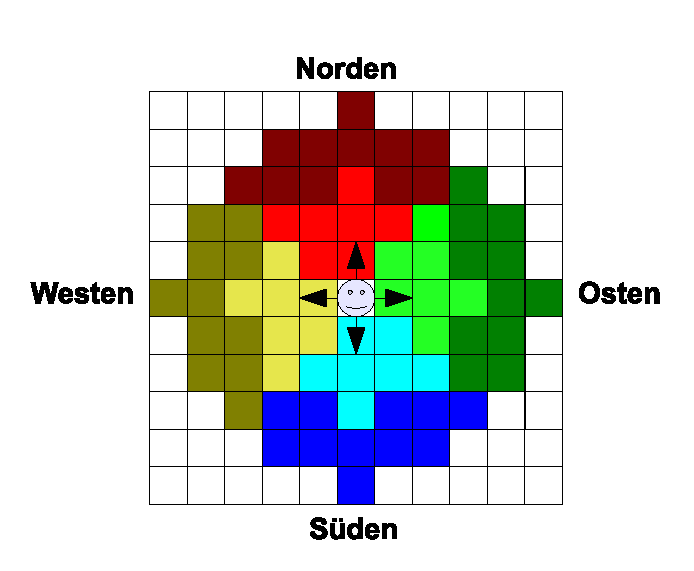
\includegraphics{sight_directions.eps}
}
\caption[Sicht- und �berwachungsreichweite eines Agenten]{Sicht- (2.0) und �berwachungsreichweite (5.0) eines Agenten, jeweils f�r die einzelnen Richtungen}
\label{sight_directions:fig}
\end{figure}

\section{F�higkeiten}\label{agent_abilities:sec}

Jeder Agent kann in jedem Schritt zwischen vier verschiedenen Aktionen w�hlen, die den vier Richtungen (Norden, Osten, S�den, Westen), bei der der Agent sich nicht bewegt, entsprechen. Agenten k�nnen pro Zeiteinheit genau einen Schritt durchf�hren. Das Zielobjekt kann je nach Szenarioparameter mehrere Schritte ausf�hren.

\section{Ablauf der Bewegung}
Alle Agenten werden nacheinander in der Art abgearbeitet, dass der jeweilige Agent die aktuellen Sensordaten aus der Umgebung holt und anhand dieser die n�chste Aktion bestimmt. Ung�ltige Aktionen, d.h. der Versuch sich auf ein besetztes Feld zu bewegen, schlagen fehl und der Agent f�hrt in diesem Schritt keine Aktion aus, wird aber nicht weiter bestraft. Eine detaillierte Beschreibung der Bewegung im Kontext anderer Agenten und Programmteile wird in Kapitel~\ref{reihenfolge:sec} gegeben.

\section{Grunds�tzliche Algorithmen der Agenten}

Neben denjenigen Algorithmen, die auf LCS basieren und in Kapitel~\ref{lcs:cha} besprochen werden, gibt es folgende Grundtypen, die dazu dienen, die Qualit�t der anderen Algorithmen einzuordnen. Wesentliches Merkmal im Vergleich zu auf LCS basierenden Algorithmen ist, dass sie statische, handgeschriebene Regeln benutzen und den Erfolg oder Misserfolg ihrer Aktionen ignorieren, d.h. ihre Regeln nicht anpassen.

\subsection{``Zuf�lliger Algorithmus''}\label{randomized_movement:sec}
Bei diesem Algorithmus wird in jedem Schritt wird eine zuf�llige Aktion ausgef�hrt. Abbildung ~(\ref{agent_random:fig}) zeigt eine Beispielsituation bei der der Agent jegliche Sensordaten ignoriert und eine Aktion zuf�llig ausw�hlen wird.

\begin{figure}[htbp]
\centerline{	
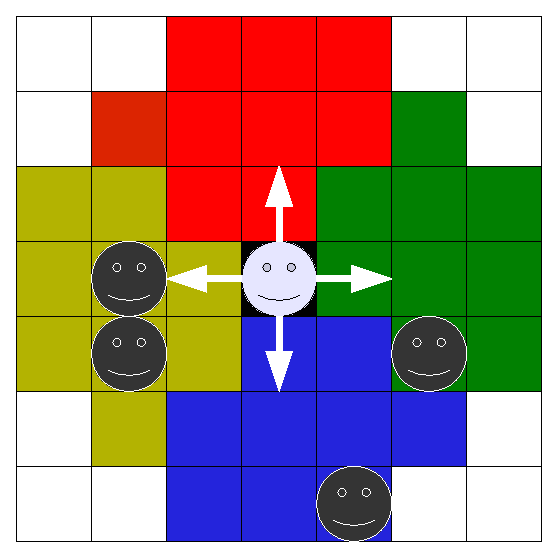
\includegraphics{agent_random.eps}
}
\caption[Sich zuf�llig bewegender Agent]{Agent bewegt sich in eine zuf�llige Richtung (oder bleibt stehen)}
\label{agent_random:fig}
\end{figure}

\subsection{Einfache Heuristik}\label{simple_heuristik:sec}
Ist das Zielobjekt in Sichtweite, bewegt sich ein Agent mit dieser Heuristik  auf das Zielobjekt zu, ist es nicht in Sichtweite, f�hrt er eine zuf�llige Aktion aus. Abbildung ~(\ref{simple_agent_to_goal:fig}) zeigt eine Beispielsituation bei der sich das Zielobjekt (Stern) im S�den befindet, der Agent mit einfacher Heuristik die anderen Agenten ignoriert und sich auf das Ziel zubewegen m�chte. 

\begin{figure}[htbp]
\centerline{	
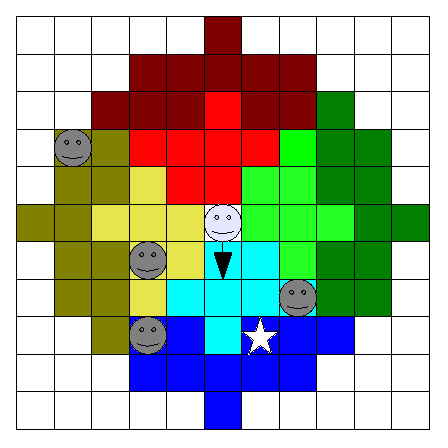
\includegraphics{simple_agent_to_goal.eps}
}
\caption[Agent mit einfacher Heuristik]{Agent mit einfacher Heuristik: Sofern es sichtbar ist bewegt sich der Agent auf das Zielobjekt zu.}
\label{simple_agent_to_goal:fig}
\end{figure}

\subsection{Intelligente Heuristik}\label{intelligent_heuristik:sec}
Ist der Zielobjekt in Sicht, verh�lt sich diese Heuristik wie die einfache Heuristik. Ist das Zielobjekt dagegen nicht in Sicht, wird versucht, anderen Agenten auszuweichen, um ein m�glichst breit gestreutes Netz aus Agenten aufzubauen. In der Implementation hei�t das, dass unter allen Richtungen, in denen kein anderer Agent gesichtet wurde, eine Richtung zuf�llig ausgew�hlt wird und falls alle Richtungen belegt (oder alle frei) sind, wird aus allen Richtungen eine zuf�llig ausgew�hlt wird. In Abbildung~(\ref{intelligent_agent:fig}) sieht der Agent das Zielobjekt nicht und w�hlt deswegen eine Richtung, in der die Sensoren keine Agenten anzeigt, in diesem Fall Norden.

\begin{figure}[htbp]
\centerline{	
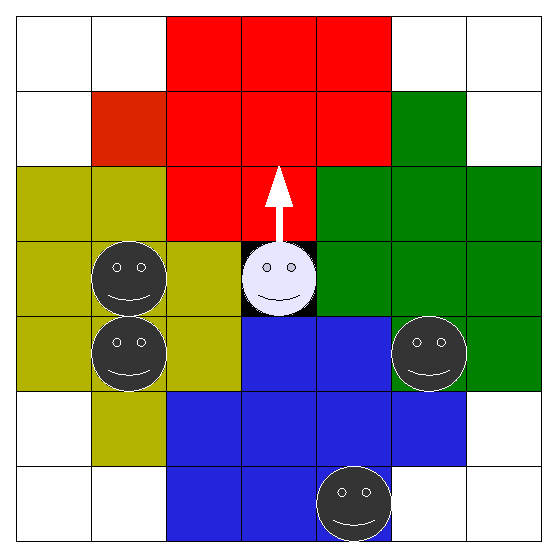
\includegraphics{intelligent_agent.eps}
}
\caption[Agent mit intelligenter Heuristik]{Agent mit intelligenter Heuristik: Falls das Zielobjekt nicht sichtbar ist bewegt sich der Agent von anderen Agenten weg.}
\label{intelligent_agent:fig}
\end{figure}
